\documentclass{article}
\usepackage[utf8]{inputenc}
\usepackage[dvipdfmx]{hyperref}
\usepackage{fancyhdr}
\usepackage{caption, floatrow}

\usepackage[dvipdfmx]{graphicx}

\usepackage{mathtools}
\renewcommand{\theequation}{eq. \arabic{equation}}


\usepackage[
  style=numeric,
  citestyle=numeric,
  url=true,
  doi=false,
  isbn=false
  ]{biblatex}
\addbibresource{main.bib}


\DeclareNewFloatType{graph}{placement=H, name=Graph}
\floatsetup[graph]{capposition=bottom}


% contents below
% ------------------------------------------------------------------------------

\pagestyle{fancy}
\fancyhf{}
\rhead{Rikuo Hasegawa}
\chead{UPCSE PHYSICS Long Lab Report}
\lhead{\today}
\rfoot{p. \thepage}

\title{Measurement of the Latent Heat of Evaporation of Liquid Nitrogen via Observations of its Mass at Room Temperature}
\author{ Rikuo Hasegawa
  \\ Tutorial Group: C
  \\ Lab Group: C2
  \\ Lab Pair: Mohammed Alsaleh}

\begin{document}

\maketitle
\thispagestyle{fancy}
\vspace*{\fill}
\parbox{\linewidth}{\centering%
Date of Experiment: March 6, 2019
\\ Date of Report Submission: March 20, 2019
\\ UCL Undergraduate Preparatory Certificate for Science and Engineering
}
\newpage

\section*{Abstract}
\paragraph{}

The aim of this experiment was to measure the latent heat of evaporation for liquid nitrogen, which is known to be $5.59 \text{kJ/mol}$ according to the literature \autocite{mohr_2016}. Unfortunately, the experiment measure the following values which do not coincide with this known value:

\begin{align*}
  L_{\text{with outliers}}    &= 13.2 \pm 5.67 ~ \text{[kJ/mol]} \\
  L_{\text{without outliers}} &= 7.84 \pm 0.46 ~ \text{[kJ/mol]}
\end{align*}

In this report, we introduce the theory behind latent heat. Then, we explain the experiment apparatus and protocol. This is followed by an analysis of our results. Finally, we will discuss our results and give our conclusion.

\section{Introduction}

\subsection{Theory}
\paragraph{}

When matter receives heat energy, its temperature will rise. At some point, it will stop rising in temperature and instead undergo a phase transition. A phase transition from liquid to gas is called evaporation, which occurs when the material's temperature is at its boiling point. Phase transitions require energy which is used to free each molecule from its bound state. The energy required per unit mass of some uniform material to completely undergo a phase transition is called the Latent heat ($L$). The relation to the energy $Q$ and mass $m$ is linear as shown in \eqref{eq:latent}.

\begin{equation}\label{eq:latent}
  Q = Lm
\end{equation}

By taking the derivative on both sides of the equation, we get \eqref{eq:power}.

\begin{equation}\label{eq:power}
  P = \frac{dQ}{dt} = L \frac{dm}{dt}
\end{equation}

When conducting an experiment in an environment where the background temperature is different from the temperature of the substance's boiling point, heat is either gained or lost into the background environment ($Q_b$, or $P_b$). We can apply a known constant power source $P$ to the same material, which allows us to remove the background heat loss from the equation, giving us \eqref{eq:lab_book} where $\left( \frac{dm}{dt} \right)_b$ is the rate of decrease of mass when the liquid nitrogen is exposed to only background heat, and $\left( \frac{dm}{dt} \right)_h$ is the same rate when it is exposed to both the background heat and the heat from a power source.

\begin{align}
\begin{split}
  P_{b} = L \left( \frac{dm}{dt} \right)_b \\
  P + P_b = L \left( \frac{dm}{dt} \right)_h
\end{split}
\begin{split}\label{eq:lab_book}
  \frac{P}{L} = \left( \frac{dm}{dt} \right)_h - \left( \frac{dm}{dt} \right)_b
\end{split}
\end{align}

With a simple circuit connected to a resistor, the power output of the resistor $P$ can be expressed in terms of the voltage and current of the power source.

\begin{equation}\label{eq:resistor}
  P = VI
\end{equation}

Thus, the latent heat of evaporation of some material can be expressed as \eqref{eq:final}.

\begin{equation}\label{eq:final}
  L = \cfrac{VI}{\left( \frac{dm}{dt} \right)_h - \left( \frac{dm}{dt} \right)_b}
\end{equation}

\subsection{Aims and Objectives}
\paragraph{}

The aim of this experiment is to find the latent heat of evaporation for liquid nitrogen. In order to do this, we will measure the rate of decrease of mass as liquid nitrogen evaporates in room temperature, with and without a heat source applied to it.

\section{Experimental Equipment and Method}
\subsection{Apparatus}
\paragraph{}
The apparatus is shown in Figure \ref{fig:apparatus}. The main components are listed below:

\begin{itemize}
  \item liquid nitrogen and bowl
  \item lid with resistor
  \item stopwatch
  \item voltmeter (uncertainty: 0.005 V)
  \item ammeter (uncertainty: 0.005 A)
  \item DC power source
  \item scale (uncertainty: 0.05 g)
\end{itemize}

\begin{figure}[H]
  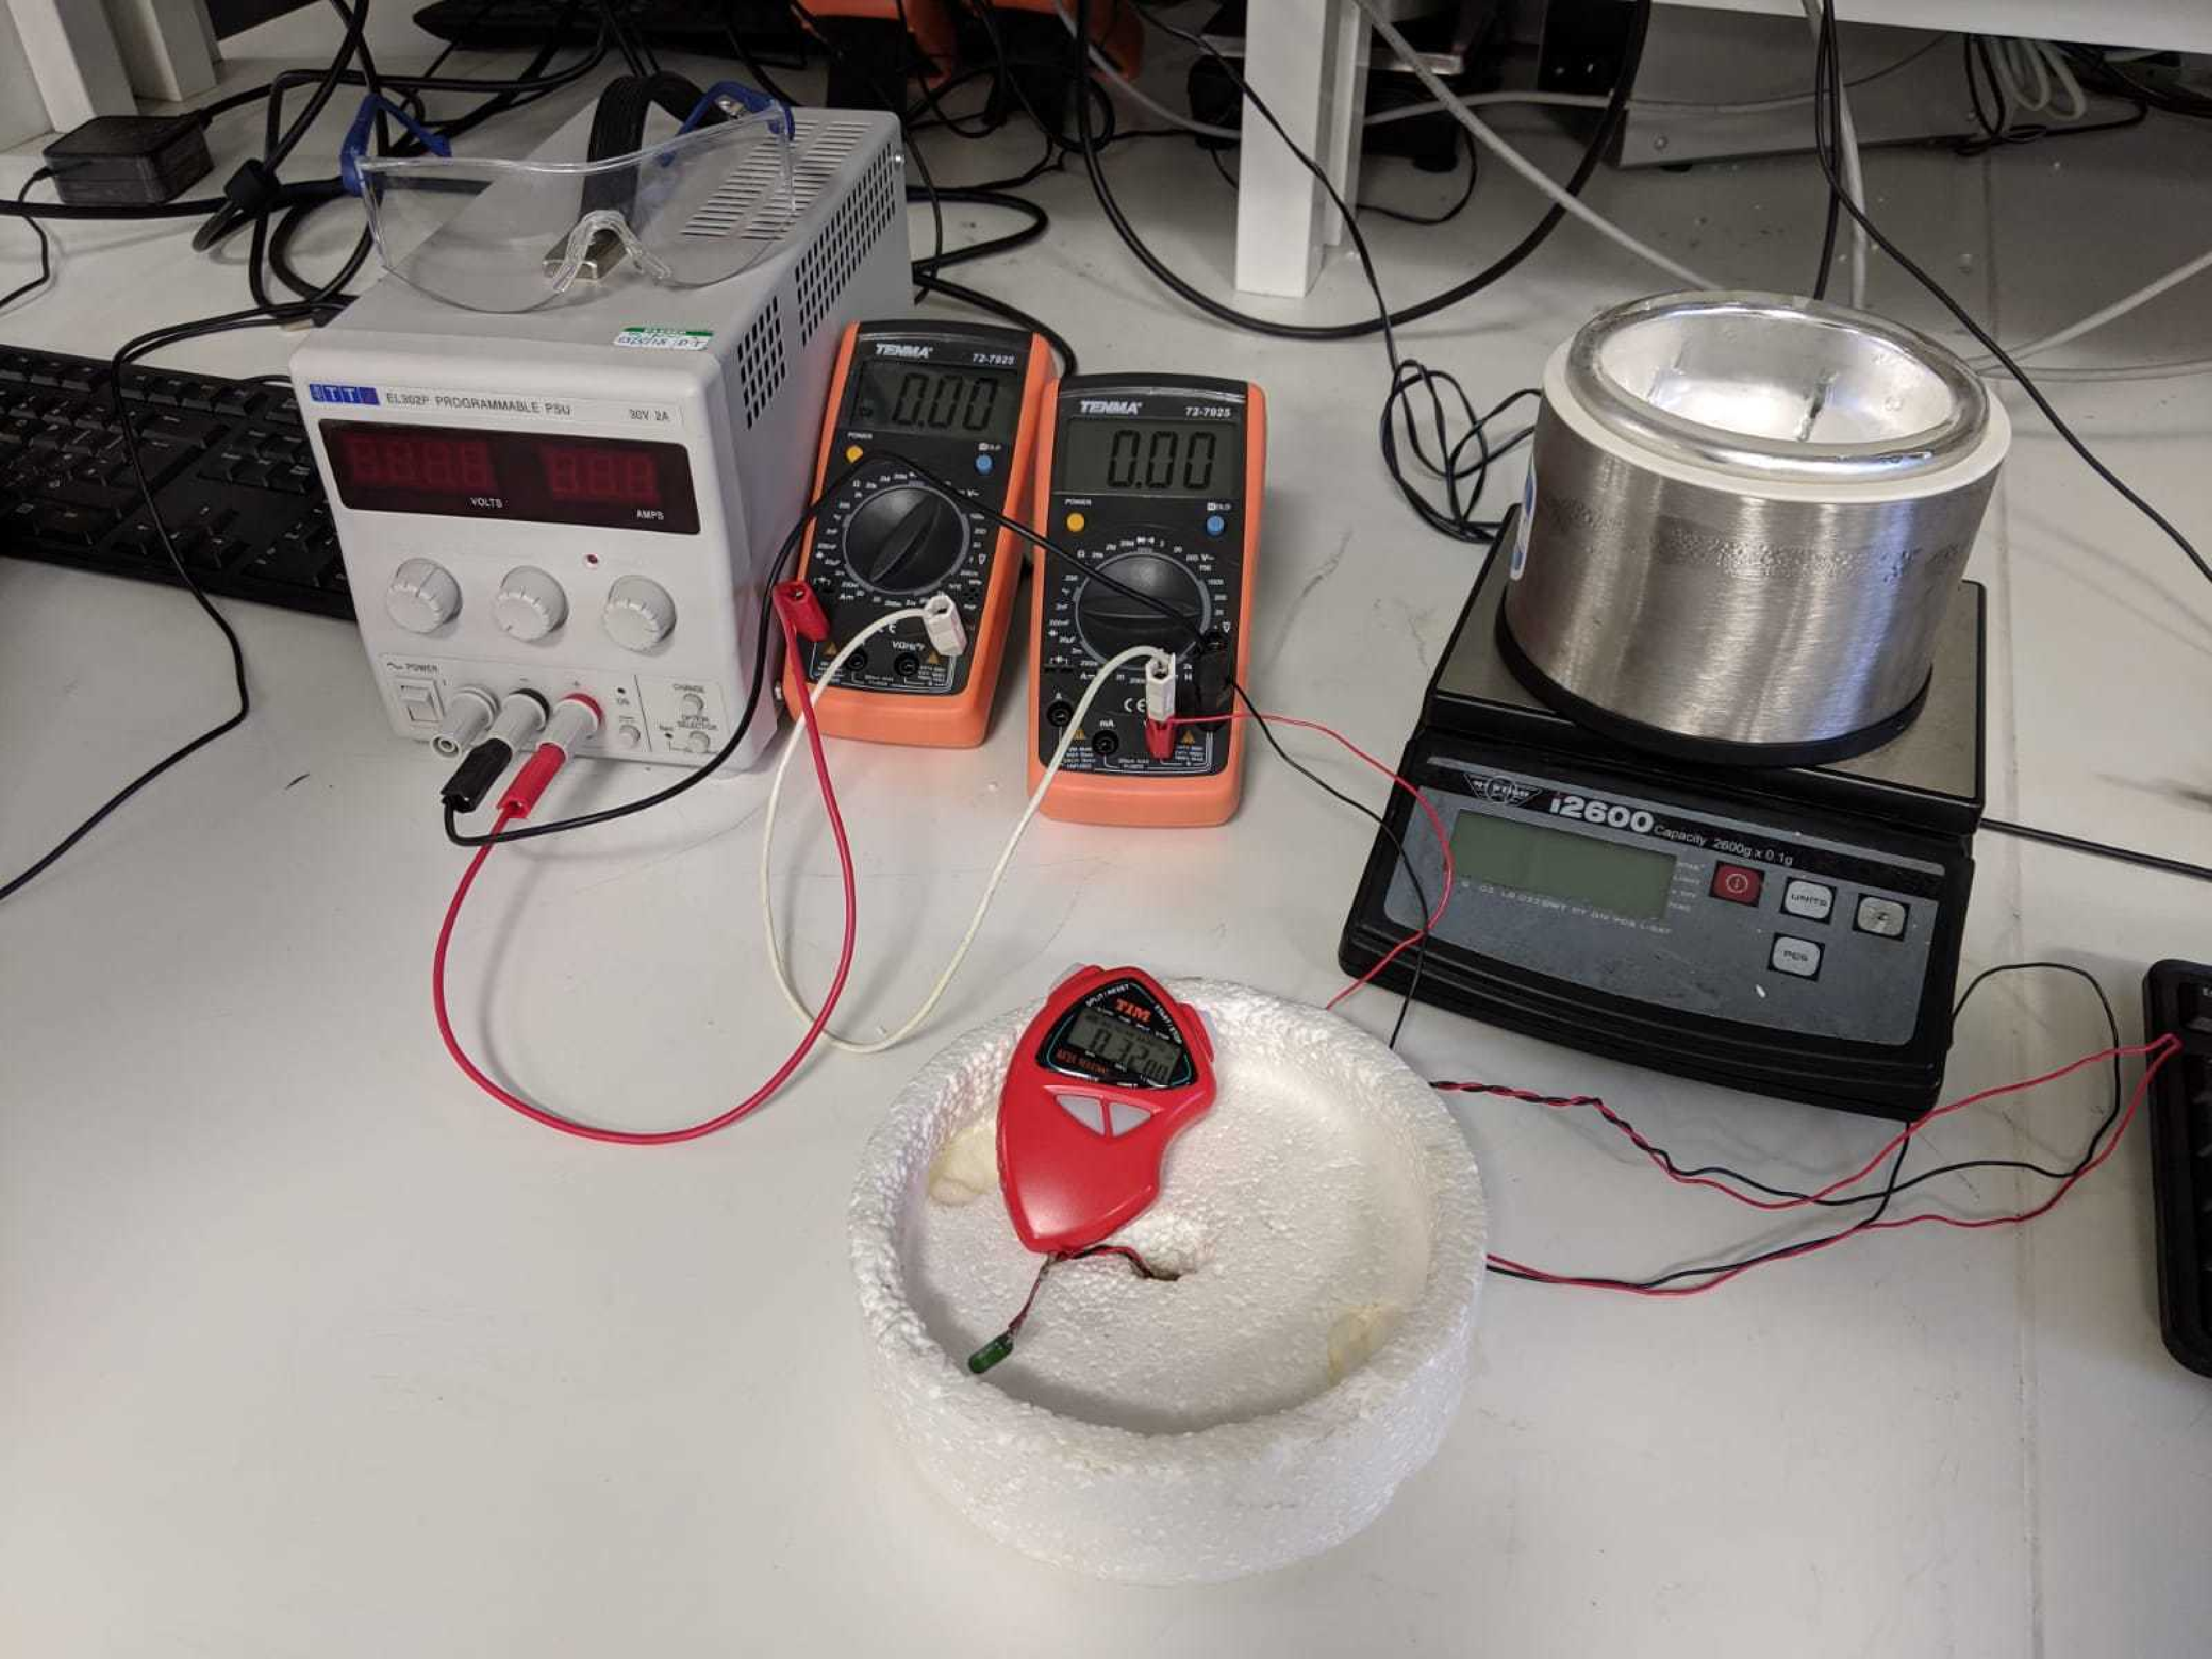
\includegraphics[width=\textwidth]{./img/apparatus.pdf}
  \caption{Experiment setup. The metal bowl to hold the liquid nitrogen is placed on top of a scale. The foam lid has a hole for the wiring of the resistor.}
  \label{fig:apparatus}
\end{figure}

The DC power source, ammeter, voltmeter, and resistor are connected according to the following circuit shown in Figure \ref{fig:circuit}.

\begin{figure}[H]
  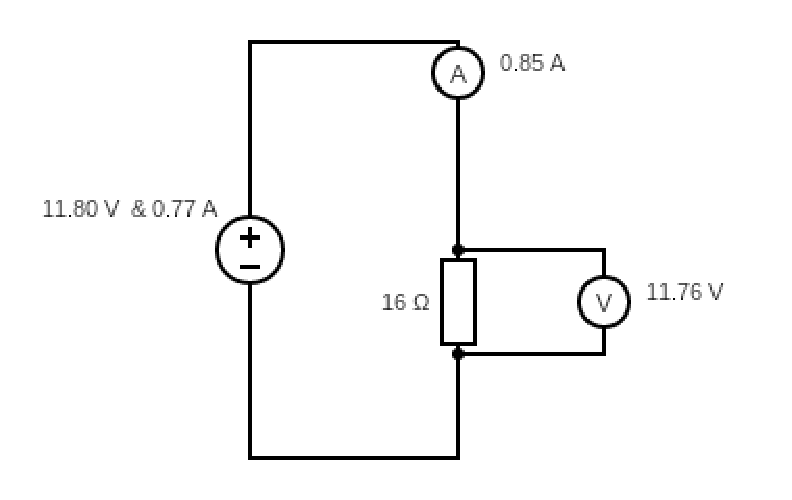
\includegraphics[width=\textwidth]{./img/circuit.pdf}
  \caption{The electronic circuit with the observed values of current and voltage. Note the reading on the voltmeter/ammeter differ slightly from the reading on the power source. This could be because the wires and connections have non-zero resistance or the power source is not calibrated accurately.}
  \label{fig:circuit}
\end{figure}

\subsection{Protocol}
\paragraph{}
The experimental protocol is described below.

\begin{enumerate}
  \item Zero the scale with the bowl on the scale.
  \item Pour slightly more than 200g of liquid nitrogen into the bowl.
  \item When the scale reads 200.0 g, start the stopwatch.
  \item Loop. This gives us $m_{b1}(t)$.
    \begin{enumerate}
      \item When $t ~\%~ 30 ~\text{[sec]} = 0$, record the reading on the scale.
      \item If $t = 300 ~\text{[sec]}$ exit the loop.
    \end{enumerate}
  \item Turn on the DC power source, voltmeter, and ammeter such that $P = 10 [W]$. (Shown in Figure \ref{fig:circuit})
  \item Repeat the loop. This gives us $m_h(t)$
  \item Turn off the DC power source.
  \item Repeat the loop. This gives us $m_{b2}(t)$.
\end{enumerate}

We get two measurements for the mass decrease with background heat since we may find that the background heat is not constant throughout the experiment, or it is affected by turning the DC power source on. If we take the average of the decrease in mass due to background heat before and after we add more heat and use that for our mass decrease under background heat, we may be able to lessen the effect this has on our measurement.

\section{Measurements and Results}
\paragraph{}

Our raw measurements for the mass at each point in the experiment is shown in Table \ref{tb:raw}. Looking at \eqref{eq:final}, since $L$ is a constant for a material, the rate of decrease of mass should be linear with respect to time (i.e. $\left( \frac{dm}{dt} \right) = c$ where $c$ is some constant). The latent heat $L$ can be determined by the power output of the resistor, 10 Watts, and the difference of the gradient of the line with the heater on, and with the heater off.

\begin{table}[H]
\begin{tabular}{|c|c|c|c|}
\hline
\textbf{$t$ [sec]} & \textbf{$m_{b1}$ [g]} & \textbf{$m_h$ [g]} & \textbf{$m_{b2}$ [g]} \\ \hline
\textbf{0}              & 200.0                  & 160.0                 & 138.0                  \\ \hline
\textbf{30}             & 182.4                  & 158.1                 & 137.5                  \\ \hline
\textbf{60}             & 180                    & 156.1                 & 136.9                  \\ \hline
\textbf{90}             & 178.4                  & 154.1                 & 136.3                  \\ \hline
\textbf{120}            & 177.2                  & 152.2                 & 135.8                  \\ \hline
\textbf{150}            & 176.1                  & 150.3                 & 135.2                  \\ \hline
\textbf{180}            & 175.3                  & 148.4                 & 134.7                  \\ \hline
\textbf{210}            & 174.3                  & 146.6                 & 134.1                  \\ \hline
\textbf{240}            & 173.4                  & 144.8                 & 133.6                  \\ \hline
\textbf{270}            & 172.5                  & 143                   & 132.9                  \\ \hline
\textbf{300}            & 171.7                  & 141.3                 & 132.3                  \\ \hline
\end{tabular}
\caption{Raw measurement of the mass of the liquid nitrogen in the bowl for each loop.}
\label{tb:raw}
\end{table}

Our results are plotted in Graph \ref{graph:mass}. There are a couple things to note here.

First, the gradient for the line with the heater on has a greater magnitude compared to the gradient without the heater on as expected, minus one caveat, which is the second thing to note.

There are some outliers in the graph at the beginning of the line for $m_{b1}$, where the mass decreased much rapidly compared to everywhere else in the graph. This is most likely due to the fact that we only applied slightly more than 200g of liquid nitrogen to the bowl, which was near room temperature. Thus, the initial background heat loss is due to a combination of the bowl's heat as well as the heat lost to the air at the surface of the liquid. As the bowl cooled to a temperature close to that of the liquid nitrogen, the background heat loss is mainly due to only the heat lost at the surface.

\begin{graph}[H]
  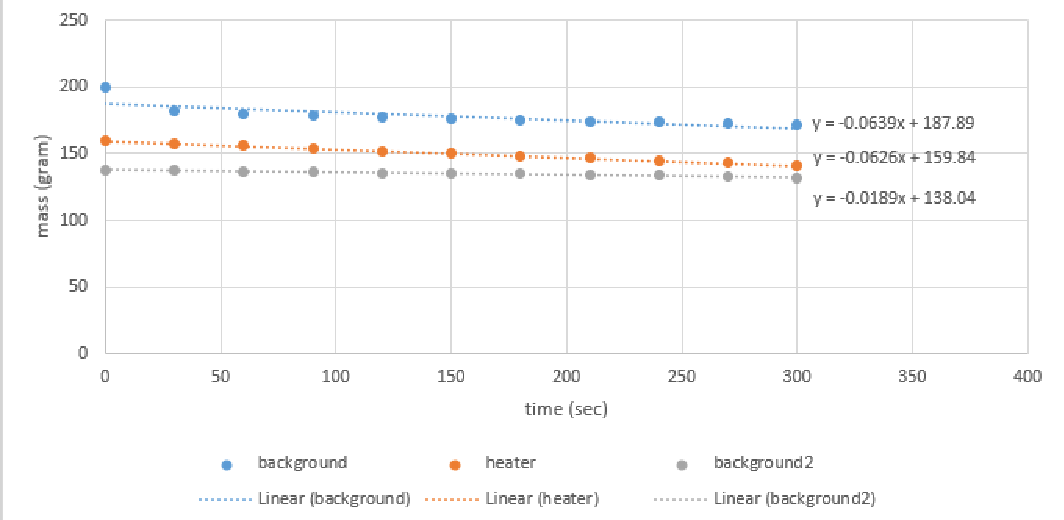
\includegraphics[width=\textwidth]{./img/graph.pdf}
  \caption{Mass lost due to evaporation over time.}
  \label{graph:mass}
\end{graph}

Using the regression tool in Microsoft Excel's Data Analysis Toolkit, we obtain the following values for the rate of loss of mass and their uncertainties depending on whether we accept the outlier values in the beginning of the first background heat measurements.
\begin{align*}
  \Delta \left( \frac{dm}{dt} \right)_{\text{with outliers}} &=  ~0.01773 ~\text{[g/s]}\\
  \left( \frac{dm}{dt} \right)_{\text{with outliers}} &= -0.04141 ~\text{[g/s]}\\
  \Delta \left( \frac{dm}{dt} \right)_{\text{without outliers}} &= ~0.001448 ~\text{[g/s]}\\
  \left( \frac{dm}{dt} \right)_{\text{without outliers}} &= -0.02488 ~\text{[g/s]}
\end{align*}

Using \eqref{eq:final}, we can calculate the uncertainty on our measurements using \eqref{eq:u_product} and \eqref{eq:u_sum}  for combining uncertainties when the combination of values takes on a function $f$ which is either a product or sum of values \autocite{Palmer}.

\begin{align}
  \label{eq:u_product} f = ax + by &\to \Delta f = \sqrt{a^2\Delta x^2 + b^2 \Delta y^2}\\
  \label{eq:u_sum} f = kx^{n_1}y^{n_2} &\to \frac{\Delta f}{f} = \sqrt{n_1^2 \left( \frac{\Delta x}{x} \right)^2 + n_2^2 \left( \frac{\Delta y}{y} \right)^2}
\end{align}

The working of how one can arrive at \eqref{eq:uncertainty} which gives us the uncertainty of $L$ from \eqref{eq:final} is shown below:

\begin{align*}
\begin{split}
  &L = \cfrac{VI}{\frac{dm}{dt}}
  \\
  &\text{where}~ \frac{dm}{dt} = (\frac{dm}{dt})_h - (\frac{dm}{dt})_b
\end{split}
\end{align*}

\begin{align*}
  \left( \frac{dm}{dt} \right)_b &= \frac{1}{2} \left(
    \left( \frac{dm}{dt} \right)_{b1}
    + \left( \frac{dm}{dt} \right)_{b2}
    \right) ~\text{[g/s]}
  \\
  \Delta \left( \frac{dm}{dt} \right)_b &=
    \sqrt{\cfrac{
      \left( \Delta \frac{dm}{dt} \right)^2_{b1} + \left( \Delta \frac{dm}{dt} \right)^2_{b2}
    }{4}}
  \\
  \Delta \frac{dm}{dt} &= \sqrt{ \left( \Delta \frac{dm}{dt} \right)^2_h + \left( \Delta \frac{dm}{dt} \right)^2_b }
  \\
  \Delta V &= 0.005 ~\text{[V]}
  \\
  \Delta I &= 0.005 ~\text{[A]}
\end{align*}

\begin{equation}\label{eq:uncertainty}
  \frac{\Delta L}{L} = \sqrt{ \left( \frac{0.005}{11.76} \right)^2 + \left( \frac{0.005}{0.85} \right)^2 + \left( \frac{\Delta \frac{dm}{dt}}{\frac{dm}{dt}} \right)^2 } ~\text{[kJ/kg]}
\end{equation}

Plugging these into \eqref{eq:uncertainty}, we get the following values for the latent heat of evaporation for liquid nitrogen:

\begin{align*}
  L_{\text{with outliers}}    &= 471.8 \pm 202.0 ~ \text{[kJ/kg]} \\
  L_{\text{without outliers}} &= 280.0 \pm 16.4 ~ \text{[kJ/kg]}
\end{align*}

Converting these values into [kJ/mol] using the knowledge that the molar mass of nitrogen is 28.0 g \autocite{UPCSE2018}, we get the following values:

\begin{align*}
  L_{\text{with outliers}}    &= 13.2 \pm 5.67 ~ \text{[kJ/mol]} \\
  L_{\text{without outliers}} &= 7.84 \pm 0.46 ~ \text{[kJ/mol]}
\end{align*}

Unfortunately, neither value is within the range of the true value of the latent heat of evaporation for liquid nitrogen, 5.59 [kJ/mol].


\section{Discussion and Conclusion}
\paragraph{}

The aim of this experiment was to measure the latent heat of evaporation of liquid nitrogen. The results are summarized below:

\begin{align*}
  L_{\text{with outliers}}    &= 13.2 \pm 5.67 ~ \text{[kJ/mol]} \\
  L_{\text{without outliers}} &= 7.84 \pm 0.46 ~ \text{[kJ/mol]}
\end{align*}

Unfortunately, the experiment did not successfully measure the value to an acceptable precision or accuracy, based on the true value from the literature.

The high uncertainty when keeping outlier data is to be expected, as our assumption that the background heat will remain constant throughout the experiment did not hold, causing the rate of decrease in mass to be linear. Since we continued to assume that it was linear, which caused our uncertainty to rise since the regression will search for the closest linear function to approximate the data.

However, even after removing the outlier data, we still notice systematic errors in our experiment. A potential cause for this systematic error is that the liquid nitrogen was not pure, so our measurements were correct but with respect to a mixture of various liquids (i.e. liquid oxygen). However, this is unlikely since liquid nitrogen can be manufactured with a high purity (1ppm impurity).

Another potential cause of systematic error is that the background heat is a non-linear function even after the bowl has been cooled to near equilibrium with the liquid. We see traces of this when we look at the gradient of the lines after removing the obvious outliers. $\left( \frac{dm}{dt} \right)_{b1} >   \left( \frac{dm}{dt} \right)_{b2}$ even after removing the outliers.

This experiment did not succeed in achieving its aims, but it opens the door to further research into how the background heat loss behaves, which may give us new insights into how heat can be transferred into liquid nitrogen from the environment.

\printbibliography
\end{document}
